\documentclass[11pt,a4paper]{amsart}
\usepackage{amsmath,amssymb,amsthm,mathrsfs,bm,bbm,comment}
\usepackage{xcolor}
\usepackage{pgf,tikz}
\usetikzlibrary{arrows}

\begin{document}

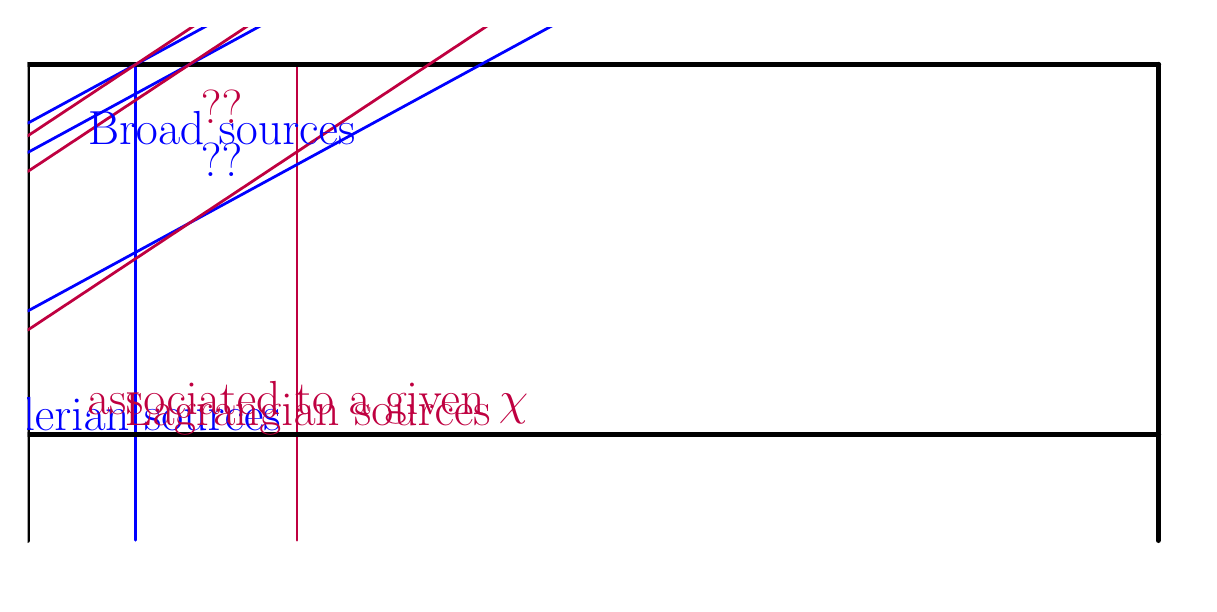
\begin{tikzpicture}[line cap=round,line join=round,>=triangle 45,x=0.683828712095508cm,y=0.671109663630229cm]
\clip(-4,-2.83) rectangle (17.56,7.7);
\draw [line width=1.pt,color=blue,fill=blue!15] (-2.,-2.) -- (-2.,7.)-- cycle;
\draw [line width=1.pt,color=purple,fill=purple!15] (1.,-2.) -- (1.,7.)-- cycle;
\draw [line width=2.pt,color=black] (-4.,0.) -- (17.,0.);
\draw [line width=2.pt,color=black] (-4.,7.) -- (17.,7.);
\draw [line width=2.pt,color=black] (-4.,-2.) -- (-4.,7.);
\draw [line width=2.pt,color=black] (17.,-2.) -- (17.,7.);
\draw [line width=1.pt,color=blue,domain=-4.:17.] plot(\x,{(--2.--\x)*tan(29)+7.});
\draw [line width=1.pt,color=purple,domain=-4.:17.] plot(\x,{(--2.--\x)*tan(34)+7.});
\draw [line width=1.pt,color=blue,domain=-4.:17.] plot(\x,{(--1.--\x)*tan(29)+7.});
\draw [line width=1.pt,color=purple,domain=-4.:17.] plot(\x,{(--1.--\x)*tan(34)+7.});
\draw [line width=1.pt,color=blue,domain=-4.:17.] plot(\x,{(--1.--\x)*tan(29)+4.});
\draw [line width=1.pt,color=purple,domain=-4.:17.] plot(\x,{(--1.--\x)*tan(34)+4.});
\draw[color=blue] (-2.2,0.4) node {\LARGE Eulerian sources};
\draw[color=purple] (1.2,0.4) node {\LARGE Lagrangian sources};
\draw[color=purple] (1.2,0.6) node {\LARGE associated to a given $\chi$};
\draw[color=blue] (-2.2,6.4) node {\LARGE \underline{}} ;
\draw[color=purple] (1.2,6.4) node {\LARGE \underline{}} ;
\draw[color=purple] (-0.4,6.2) node {\LARGE ??};
\draw[color=blue] (-0.4,5.2) node {\LARGE ??};
\draw[color=blue] (-0.4,5.8) node {\LARGE Broad sources};
\draw[color=black] (-1.3,8.2) node {\LARGE Borel, bounded functions};
\end{tikzpicture}

\end{document}